\section{Zweite Sequenz}
Auch in diesem Fall wird die Darstellung auf einen zweidimensionalen Sachverhalt reduziert.
Im vorherigen Kapitel wurde die Situation in der XY-Draufsicht analysiert.
Die folgende Untersuchung betrachtet nun die XZ-Seitenansicht.
Es soll bestimmt werden bei welchen Kombinationen aus Abfahrtswinkel und Geschwindigkeit eine Kollision mit dem Kranarm möglich ist.
Nun da der Fokus von der XY- auf die XZ-Ebene rückt, verläuft die Bewegungsbahn nicht geradlinig mehr, sondern folgt einer parabolischen Flugkurve.
%\newpage %TODO
\begin{wrapfigure}{r}{0.5\textwidth}
	\centering
	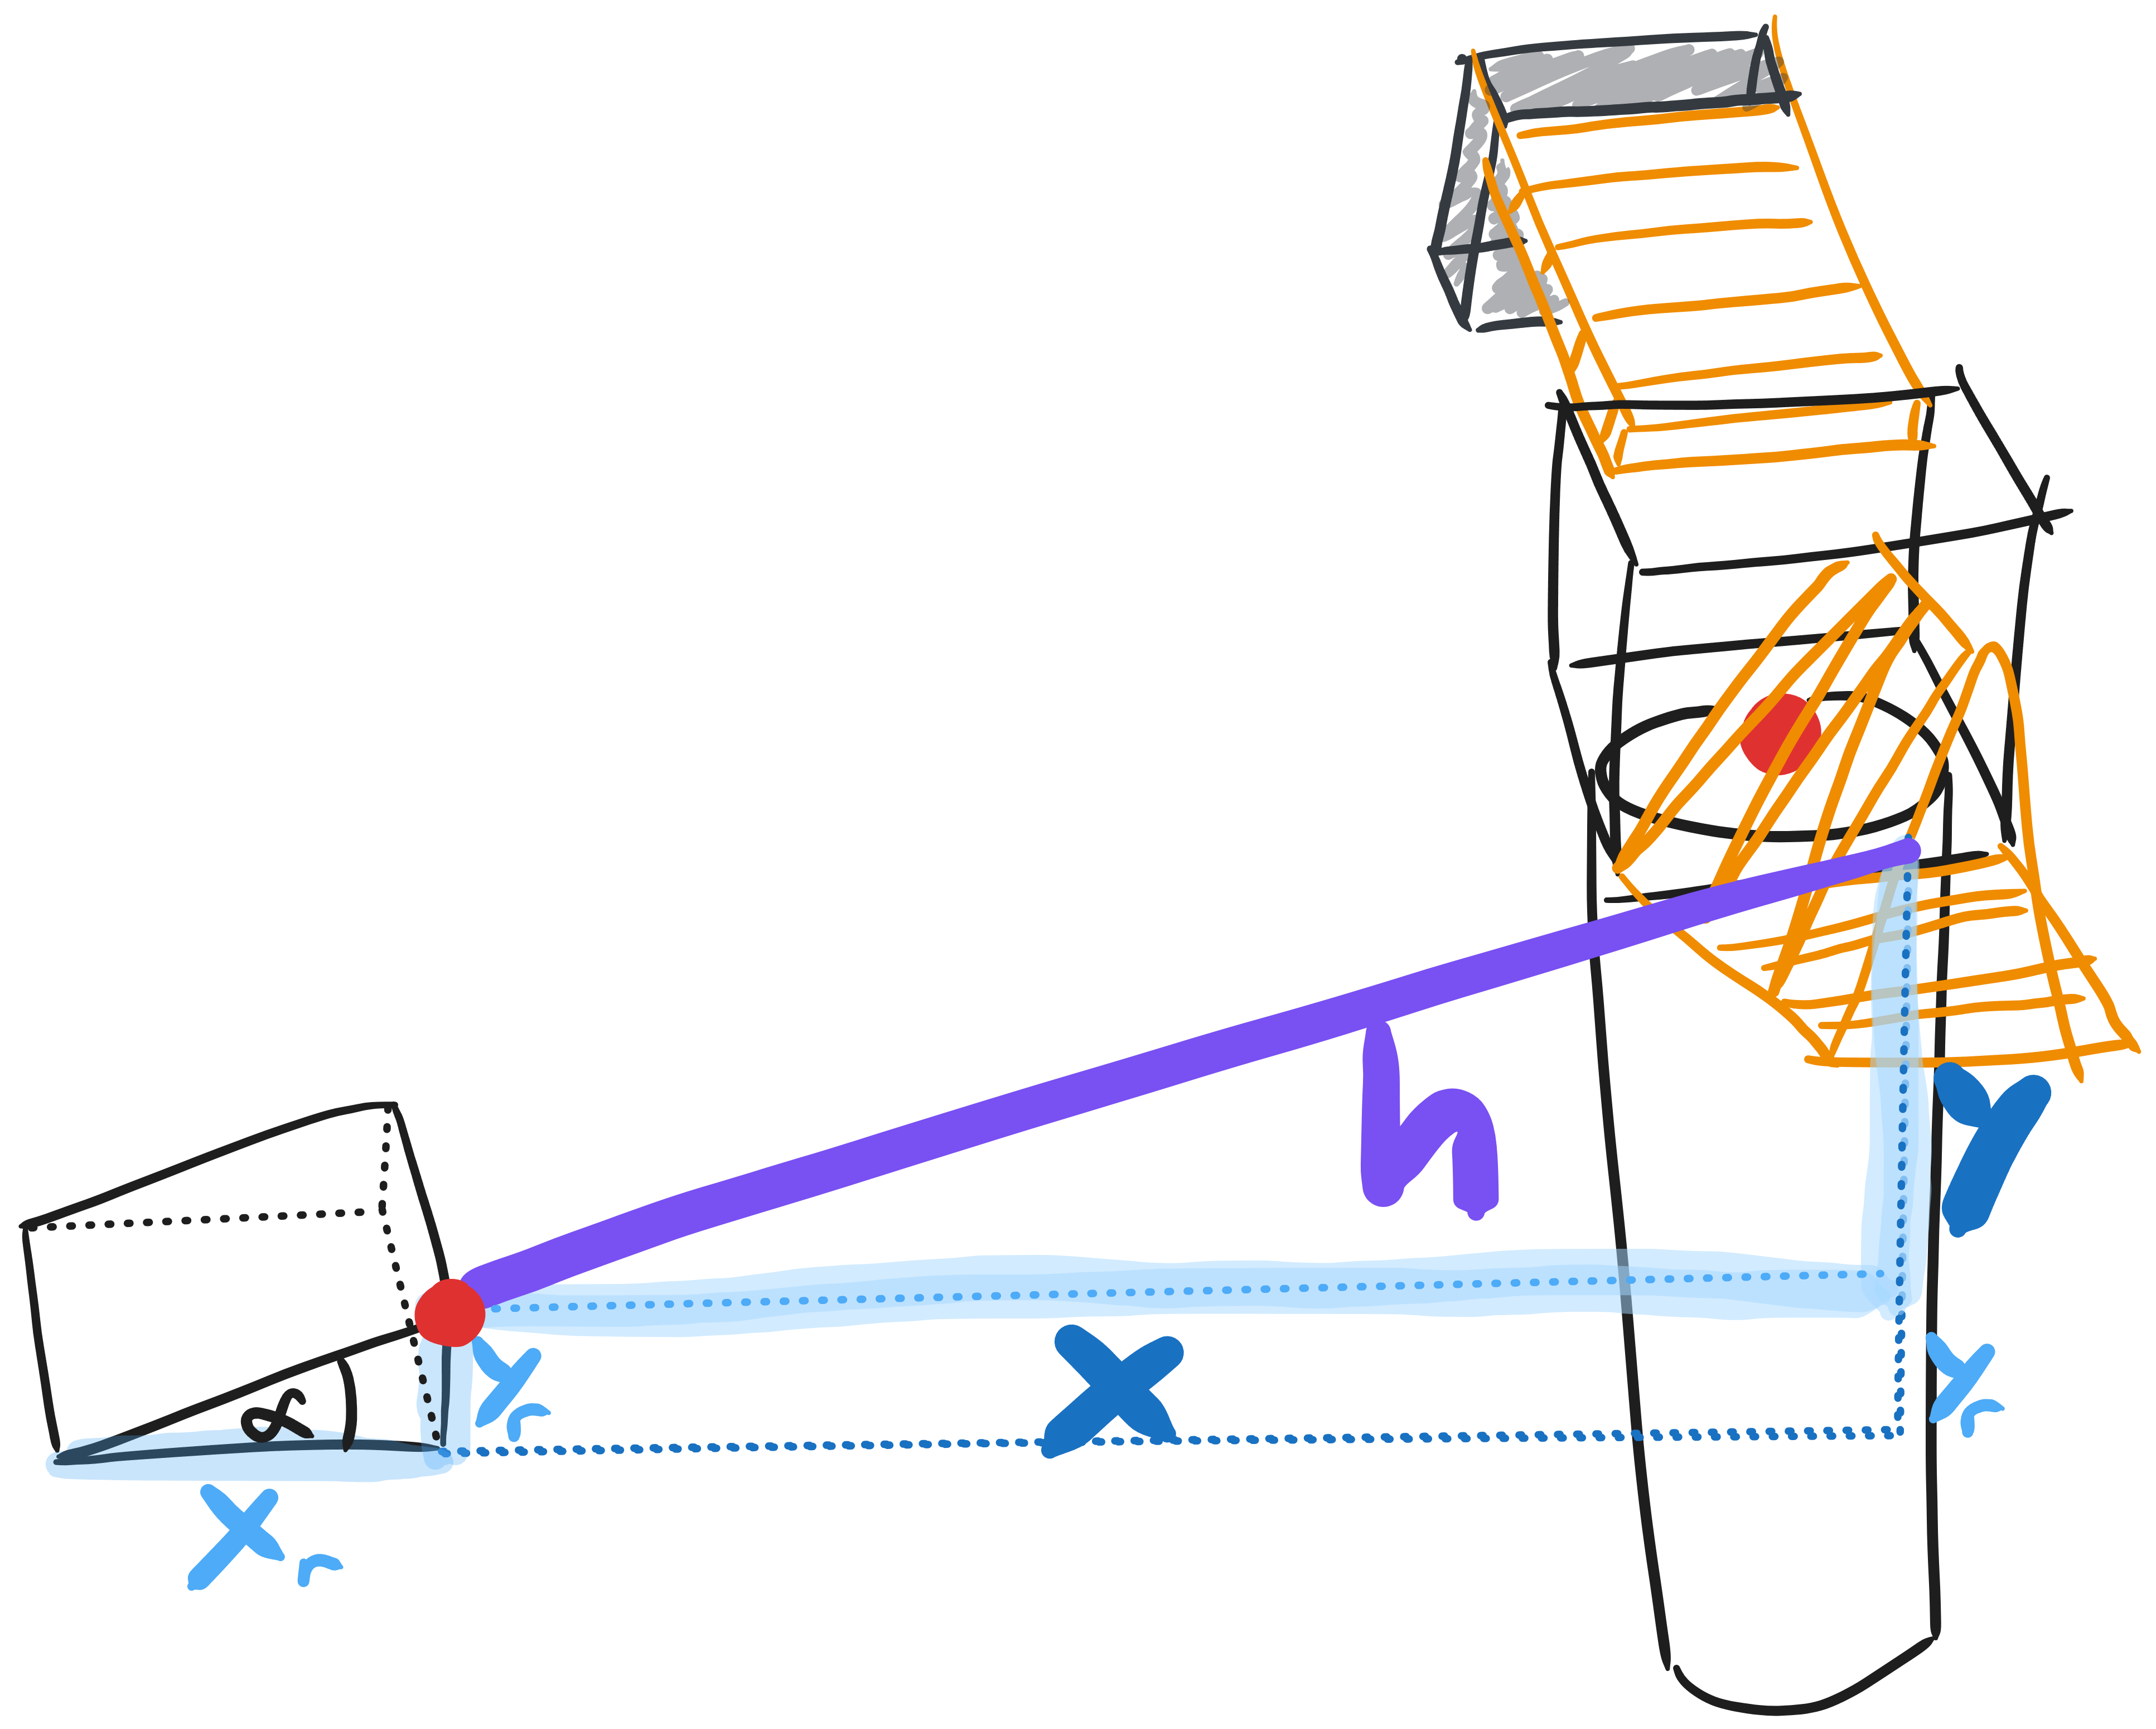
\includegraphics[width=0.48\textwidth]{resources/seq3/sketch.png}
	\vspace*{-10mm}
	\begin{flushright}
		{\scriptsize Eigenkreation; Gezeichnet in Excalidraw}
	\end{flushright}
	
	\captionsetup{
		labelfont=bf,
		textfont=footnotesize,
		skip=0pt
	}
	\caption{Skizze der zweiten Sequenz in Seitenansicht}
	\label{fig:03_xz-angle_sketch}
	%\vspace{-10pt}
\end{wrapfigure}
\hyperref[fig:03_xz-angle_sketch]{Abbildung~\ref*{fig:03_xz-angle_sketch}} zeigt die für diese Vorgang bedeutsamen Variablen. 
Die Rampenlänge und -höhe werden auf den Abschusswinkel $\alpha$ reduziert, mit 
$\alpha=\arctan(\frac{y_r}{x_r})$\\
Die in \hyperref[fig:02_xy-angle_sketch-detailed]{Abbildung~\ref*{fig:02_xy-angle_sketch-detailed}} dargestellte Strecke $t$, die das Auto in der reduzierten Draufsicht bis zur Kollision mit dem Ausleger zurücklegen muss, ist hier in \hyperref[fig:03_xz-angle_sketch]{Abbildung~\ref*{fig:03_xz-angle_sketch}} in Form der Strecke $x$ wiederzufinden.
Der Parameter $x$ wird also mit dem Wert von $t$ aus den Berechnungen der vorherigen Sequenz besetzt.
Der Wert für $y$ muss allerdings genau wie $x_r$ und $y_r$ für die Berechnungen dieser Sequenz neu geschätzt werden. %bleibt damit eine Unbekannte
$h$ Ist die direkte Strecke zwischen Rampenende und Kollisionspunkt am Ausleger.
Da die Flugbahn nur x-Richtung auf der XY-Ebene geradlinig verläuft, und nicht auch noch in y-Richtung in der XZ-Ebene\footnote{Man bemerke die Folgen meiner schlechten Namenswahl; Scheint aber unumgänglich zu sein wenn ein dreidimensionales Problem auf eine zweidimensionale Ebene, mit konventionellen Standardbeschriftungen reduziert werden, die dann von Kontext zu Kontext für unterschiedliche reduzierte Dimensionen stehen}, wird Dom sich nie direkt auf $h$ bewegen. Viel mehr suchen wir eine parabelähnliche Kurve\footnote{Gestauchte Parabel, Gedankengang erklären} die sich genau über die beiden Enden von $h$ spannt. 
Aus diesen Gründen dient $h$ nur zur groben Veranschaulichung und hat für die weiteren Rechnungen keine Relevanz. 

\subsection{Schiefer Wurf}
%TODO Quellen; Grafik 
Das physikalische Modell eines Wurfes erlaubt die Entkopplung der x- und y-Komponente. Diese beiden Bewegungen werden also völlig unabhängig voneinander und nur in Relation der Zeit als Funktionen $x(t)$ und $y(t)$ abgebildet.
\\
Unter widerstandsfreien Bedingungen enthält die Funktion $x(t)$ das grundlegende Zeit-Ort-Gesetz\parencite{WegZeitGesetzWiki}, das lediglich um einen Koeffizienten für die Berücksichtigung des Startwinkels erweitert ist. 
Dieser Koeffizient ist nötig, da wir nur den gesamten Betrag der Abschussgeschwindigkeit kennen. Durch den Winkel $\alpha$ können dann der x- und y-Betrag aus der gesamt Geschwindigkeit isoliert werden. 
\\
Die $y(t)$ Funktion verhält sich ähnlich. Als Startgeschwindigkeit wird nun allerdings die Komponente senkrecht und nicht parallel zum Boden benutzt. Um die Erdbeschleunigung zu berücksichtigen wird $\frac{1}{2}\cdot g \cdot t^2$ abgezogen.
\\
Aus der allgemeinen Startgeschwindigkeit $v_0$ in Kombination mit dem Abschusswinkel $\alpha$ folgen die horizontale und vertikale Komponente für jeweiligen x-bzw. y-Term mit: \\
$v_{0,x} = v_0\cdot\cos(\alpha)$ und
$v_{0,y} = v_0\cdot\sin(\alpha)$
\\Daraus ergibt sich:
$x(t)=v_{0,x}\cdot t$ und
$y(t)=v_{0,y}\cdot t- \frac{1}{2}\cdot g \cdot t^2$
\\
Optional ließen sich die Gleichungen um ein $+x_0$ bzw. $+y_0$ erweitern, um einen Startversatz zu akkommodieren. Da die gewählten Anfangsparameter diesen bereits implizit enthalten, wurde darauf verzichtet.
\\
Nebenbei kann man in dieser Darstellung ganz einfach qualitative Aussagen über den Hochpunkt der Flugparabel tätigen. $y(t)$ steigt so lange bis $\frac{1}{2}\cdot g\cdot t^2$ größer als $v_{0,y}\cdot t$ wird. Das passiert bei $t=\frac{v_{0,y}}{g}$.
\\
\subsubsection{Untersuchungsgegenstand und Bahnkurve}
Das Extremum der Parabel ist in diesem Kontext allerdings irrelevant. Für die Überprüfung des Realismusgrades der Sequenz ist entscheidend, dass bzw. ob es einen eindeutigen Zeitpunkt $t$ gibt, zu dem die Funktion $x(t)$ exakt den in \hyperref[fig:03_xz-angle_sketch]{Abbildung~\ref*{fig:03_xz-angle_sketch}} dargestellten Abstand $x$ annimmt und gleichzeitig die Funktion $y(t)$ den entsprechenden Wert $y$ aus der Skizze erreicht.
Anstatt dieses Problem numerisch über beispielsweise die Methode der kleinsten Schritte zu lösen, bietet es sich hier an $t$ aus beiden Teilgleichungen zu eliminieren und diese dann in Abhängigkeit von sich selbst anzugeben. \\
Um die jeweils beiden zeitabhängigen Komponenten auf eine gemeinsame Domäne zu vereinen und eine ortsbasierte Bahnkurve zu konstruieren, muss zuerst die Funktion $x(t)$ zu $t(x)$ umgekehrt werden um. Dadurch können die Funktionen $y(t)$ und $t(x)$ zu $y(t(x))$ bzw. $y(x)$ verkettet werden. Es fällt auf, dass die Höhe $y$ nun nicht mehr als Wert der Zeit, sondern als Wert der Strecke $x$ definiert ist. Die resultierende Funktion ist jetzt kein Zeit-Ort Konstrukt mehr, sondern eine rein geometrische Darstellung der Bahnkurve.
\\
Um eine Kollision nachzuweisen gilt es nun eine realistische Kombination aus Eingangsvariablen zu finden, für die die beiden Seiten der Gleichung $y(t(x_{skizze}))=y_{skizze}$ äquivalent sind. 


\subsection{Unbeschleunigte Flugkurve des Autos}
\subsubsection{Bahnkurve des unbeschleunigten schiefen Wurfs}


$y(x)=-\frac{1}{2}\cdot \frac{g}{{v_{0,x}}^2}\cdot x^2+\frac{v_{0,y}}{v_{0,x}}\cdot x$
Da $\frac{v_{0,y}}{v_{0,x}} => \frac{v_0\cdot\sin(\alpha)}{v_0\cdot\cos(\alpha)}=\tan(\alpha)$, kann $y(x)$ auch als $y(x)=-\frac{1}{2}\cdot \frac{g}{{v_{0,x}}^2}\cdot x^2+\tan(\alpha)\cdot x$ geschrieben werden.
		
\subsection{Einfluss des Lachgaseinspritzsystems}
An dieser Stelle kommt auch das aus den Filmen hinlänglich bekannte \enquote{NOS-System}(engl. \textit{Nitrous Oxide}, deutsch: Stickoxid) zum Einsatz. Während eine Lachgaseinspritzung in der Realität lediglich den Sauerstoffanteil im Brennraum erhöht und somit eine temporäre Leistungssteigerung des Motors bewirkt\parencite{NosWiki}, scheint das filmische Pendant einer gänzlich anderen Physik zu gehorchen. Dort äußert sich der Effekt in leuchtend blauen Flammen, plötzlicher Schubkraft und einer augenscheinlich vervielfachten Traktion, eine Darstellung, die eher an eine nachträglich montierte Turbine als an einen chemisch effizienteren Oxidationsprozess im Hubraum erinnert.  
\\
Im Sinne der filmischen Authentizität, werde ich die Wirkung von NOS als unmittelbare externe Beschleunigung betrachten, anstatt wie eigentlich realistisch als eine erhöhte Motorleistung.  
\\
\begin{wrapfigure}{l}{0.5\textwidth}
	\centering
	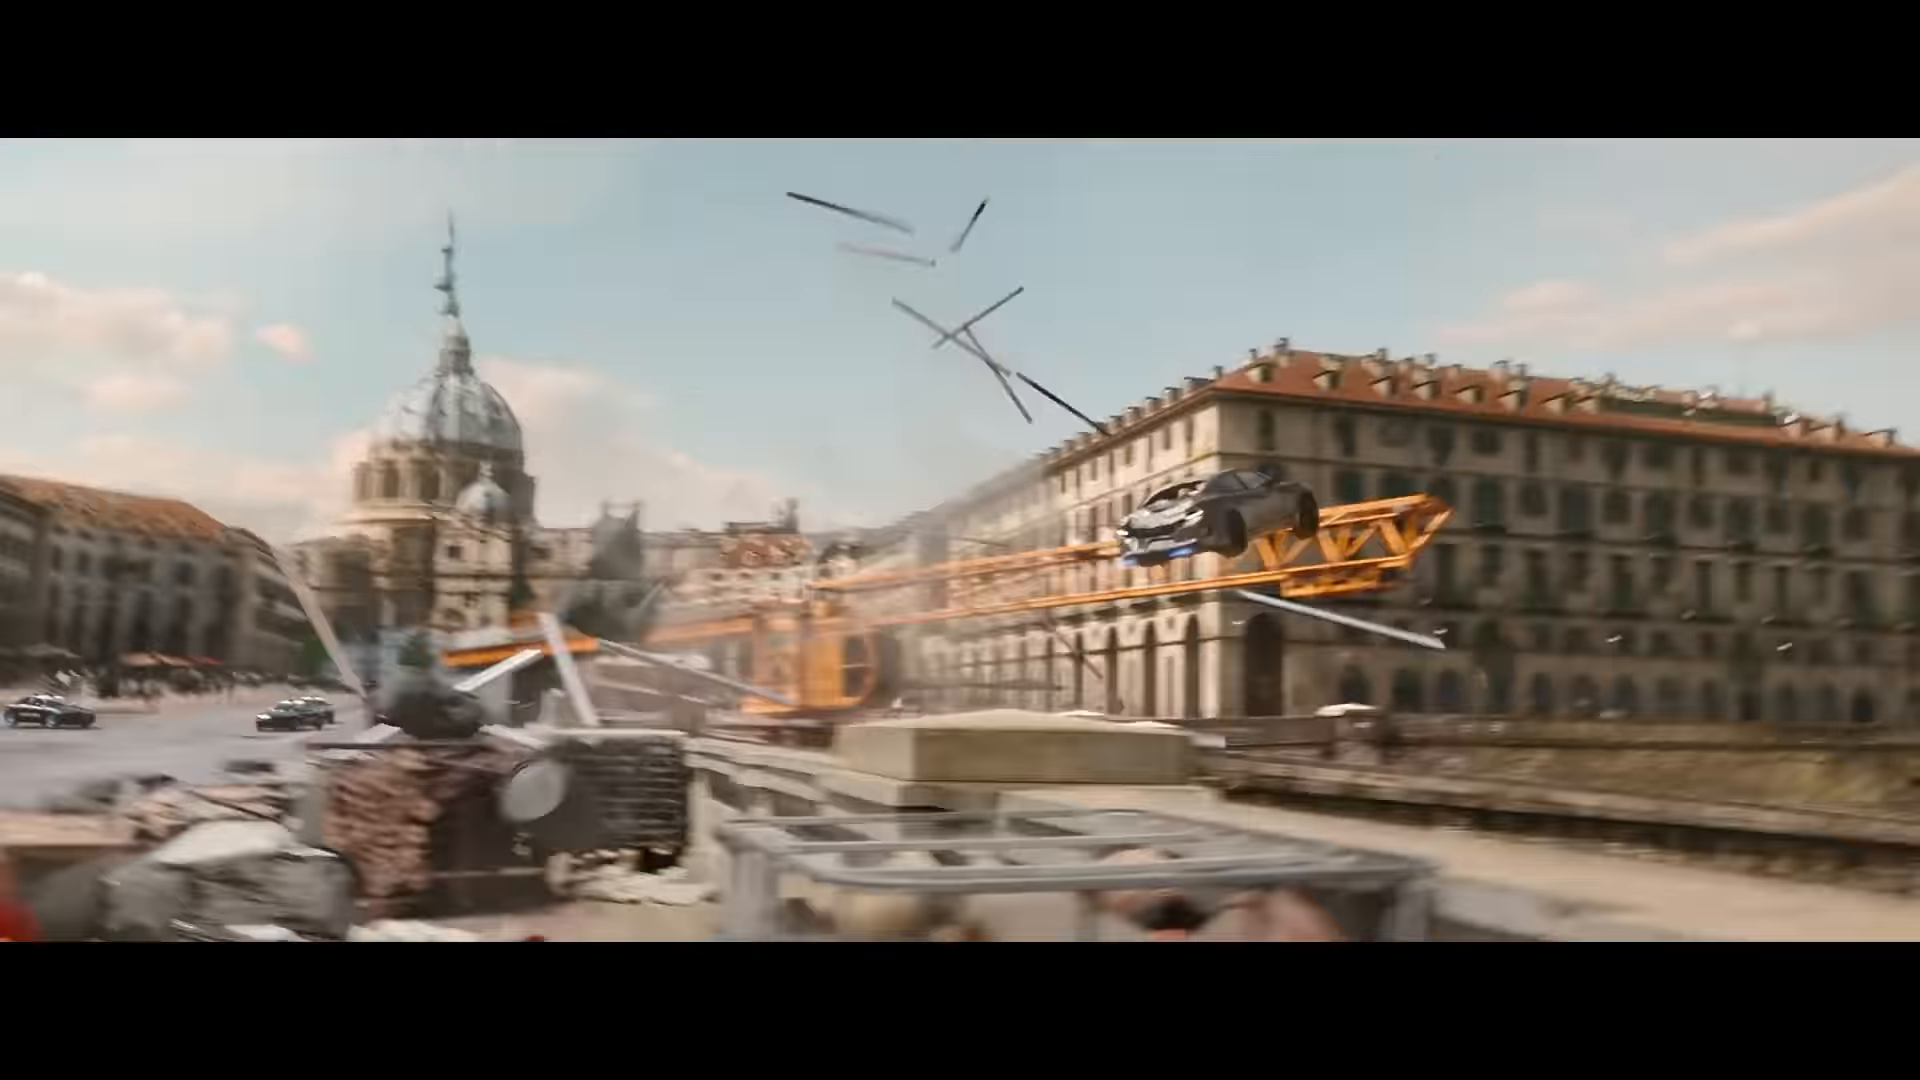
\includegraphics[width=0.48\textwidth]{resources/seq3/dom-airborne-exhaust-nitroflames-lool.png}
	\vspace*{-5mm}
	\begin{flushright}
		{\scriptsize\textcopyright\ 2023 Universal Pictures}
	\end{flushright}
	
	\captionsetup{
		labelfont=bf,
		textfont=footnotesize,
		skip=0pt
	}
	\caption{Screenshot Fast X: Dom zündet das \enquote{Lachgastriebwerk}}
	\label{fig:xy-angle_dom-pov}
	%\vspace{-10pt}
\end{wrapfigure}
\label{sec:unbeschleunigt_neigungswinkel}
Diese nicht auf Traktion beruhende Form der Kraftübertragung ermöglicht es dem Fahrzeug, selbst während der Flugphase eine zusätzliche Geschwindigkeitserhöhung zu erfahren. Zur Vereinfachung wird dieser Effekt ausschließlich auf die horizontale Komponente angewandt. Diese Annäherung entspricht offensichtlich nicht der Realität.\\
Betrachtet man die Dynamik genauer, fällt auf, dass bei sich die Fahrzeugneigung nach dem Überfahren der Rampe tatsächlich kontinuierlich ändert.
Daraus ergibt sich eine zeitabhängige Beschleunigungsrichtung. 
Intuitiv scheint es so, als ob der Fahrzeugwinkel mit der jeweils momentanen Steigung der $y(t)$ korreliert. \\
Diese Verhältnismäßigkeiten weiter zu untersuchen und korrekt zu berücksichtigen würden leider mein zeitliches Budget übersteigen, und müssen, so weh es mir tut, durch die genannte Maßnahmen approximiert werden. %TODO

\subsection{Beschleunigte Flugkurve des Autos}
Benutzt man diese Annäherung im Falle einer beschleunigten Flugphase, verhält sich die Bewegung in x-Richtung gemäß dem Weg-Zeit-Gesetz\parencite{WegZeitGesetzWiki} nicht mehr linear, sondern weist eine quadratische Abhängigkeit auf.
Die y-Komponente bleibt wie genannt unverändert, die x-Komponente wird um den Term $+\frac{1}{2}\cdot a_x\cdot t^2$ erweitert. \\
Daraus folgt:
\[
x(t)=v_{0,x}\cdot t+\frac{1}{2}\cdot a_x\cdot t^2 \qquad \text{und} \qquad
y(t)=v_{0,y}\cdot t-\frac{1}{2}\cdot g \cdot t^2
\]
\subsubsection{Bahnkurve des beschleunigten schiefen Wurfs}

\subsection{Einfluss der Aerodynamik}
Den Gegenspieler zu dieser beinahe magischen \enquote{Nitro-Beschleunigung} bildet die Bremswirkung des Luftwiderstands. 

\subsection{Gebremste Flugkurve des Autos}
Der Luftwiderstand kann grundsätzlich als lineare oder quadratische Funktion der Geschwindigkeit modelliert werden. 
Für kleine Reynolds-Zahlen $\mathrm{Re} \lesssim 1$ dominiert die viskose Reibung, und der Widerstand ist näherungsweise proportional zur Geschwindigkeit $F_L \propto v$ \parencite{owen_ryu_drag}.
Bei hohen Reynolds-Zahlen $\mathrm{Re} \gtrsim 10^3$ hingegen überwiegen trägheitsbedingte Effekte, sodass der Luftwiderstand quadratisch mit der Geschwindigkeit skaliert $F_L \propto v^2$ \parencite{owen_ryu_drag}.
Da das betrachtete Fahrzeug beim Sprung über die Rampe mit vergleichsweise hohen Geschwindigkeiten durch die Luft bewegt wird und die Reynolds-Zahl somit deutlich über $10^3$ liegt, wird in den folgenden Berechnungen der quadratische Luftwiderstand verwendet.
\[
F_L = \frac{1}{2} \cdot A \cdot \rho \cdot c_w \cdot v^2 \quad \text{\parencite{tipler_aero}}
\]
$A$ ist dabei die Frontalfläche, auf die der Luftstrom wirkt. $\rho$ steht für die momentane Luftdichte. In dieser Rechnung wird sie als konstant betrachtet. Im \textcite{tipler_aero} ist beispielsweise der Wert $1,3\frac{kg}{m^3}$ für einen \enquote{warmen Frühlingstag} gegeben.
$v$ ist der Gesamtbetrag der relativen Geschwindigkeit zwischen Oberfläche und Luftstrom und $c_w$ ist der Luftwiderstandsbeiwert. 
$c_w$ charakterisiert den strömungsbedingten Widerstand eines Körpers in Abhängigkeit von dessen Form und Oberflächenbeschaffenheit und kann ausschließlich empirisch bestimmt werden. %Wie etwa durch Windkanalversuche oder numerische Strömungssimulationen; siehe kapitel oben drüber
\\
Die Luftwiderstandskraft wirkt stets entgegengesetzt zur Bewegungsrichtung des Fahrzeugs. Das bedeutet, dass die momentane Geschwindigkeit nicht nur durch die anfänglichen Bedingungen, sondern auch durch die ständig gegenwirkende Bremskraft beeinflusst wird. Weil $F_L$ selber jedoch quadratisch mit der Gesamtgeschwindigkeit wächst, entsteht daraus ein Differentialgleichungssystem. 
\\
Der Luftwiderstand wirkt dabei in jedem Moment gegen beide, die horizontal $v_x$- und die vertikal $v_y$-Komponente.
Da die Kraft ihrerseits aber (quadratisch) von der Gesamt- und nicht von den beiden Teilgeschwindigkeiten der Komponenten abhängt, enthält nun jede der beiden Teilgleichung eine Referenz auf die jeweils andere. Das liegt an der Definition der Gesamtgeschwindigkeit mit $v = \sqrt{v_x^2 + v_y^2}$. Weil jetzt mit jeweils beiden Komponenten irgendwie das $F_L$-Konstrukt mit Abhängigkeit von gesamt $v$ verrechnet werden müsste, kommt in der Differentialgleichung des einen Teils, beispielsweise $v_x$, über das $v$ in $F_L$ dann auch der wechselseitige Term mit $v_y$ vor.
\\
Diese gegenseitige Abhängigkeit von $v_x$ und $v_y$ führt zu einem nichtlinearen gekoppelten Differentialgleichungssystem, da die Kraft in jeder Richtung von der Summe der quadratischen Beiträge beider Komponenten abhängt. 
Analytische Lösungen sind hier nicht möglich, weil sich die Geschwindigkeit in jeder Richtung gleichzeitig ändert und die quadratische Kopplung nicht in einfache Einzelgleichungen zerlegt werden kann. 
\\
\\
Um die unvermeidliche Sünde des numerischen Rechnens noch ein wenig hinauszuzögern, können unter bestimmten Annahmen Näherungen getroffen werden, die eine analytische Behandlung ermöglichen. Neben üblichen Vereinfachungen wie konstanter Luftdichte und konstantem Widerstandsbeiwert müssen noch einige weitere Maßnahmen ergriffen werden, um das System zu entkoppeln. Diese stellen aber aufgrund der augenscheinlich relativ flachen Flugkurve im Film keine großen Verzerrungen des Ergebnisses dar.
\\
Die flache Kurve entsteht durch einen sehr kleinen Flugwinkel, was bedeutet, dass die horizontale Geschwindigkeit $v_x$ den größten Teil der Gesamtgeschwindigkeit $v$ ausmacht. Dadurch gilt näherungsweise $v \approx v_x$ und die Kopplung über $v_y$ wird vernachlässigbar. Folglich spielt die vertikale Luftreibung, wie erwähnt, für das Endergebnis nur eine untergeordnete Rolle und wird der Vereinfachung halber außer Acht gelassen
\\
Ganz allgemein muss auch die Kippbewegung des Fahrzeugs, wie schon bei der \hyperref[sec:unbeschleunigt_neigungswinkel]{beschleunigten Flugkurve}, vernachlässigt werden. Dadurch wird sichergestellt, dass die Frontalfläche $A$ während des Flugverlaufs konstant bleibt.
\\
%Unter diesen Annahmen reduziert sich die Differentialgleichung für die horizontale Komponente zu einer separierbaren Gleichung:
\\
Um die Bremskraft in Abhängigkeit vom Ort ausdrücken zu können, müssen zunächst die zugrunde liegenden Bewegungsgleichungen aufgestellt werden:
\[
\dot{x} = v_x \qquad
\ddot{x} = \frac{dv_x}{dt} = a_x \qquad
\overset{\text{2. Newton}}{\Longrightarrow} \quad
m\cdot \ddot{x} = m\cdot a_x = \sum F_x
\]
Mittels Newton 2: $F=m\cdot a$ kann die Bremskraft mit $\ddot{x}$ verrechnet werden:
%Nach dem zweiten Newtonschen Gesetz $F = m \cdot a$ gilt für die horizontale Beschleunigung:
\label{sec:fall_vier_ax}
\[
m \cdot \frac{dv_x}{dt} = -\frac{1}{2} \cdot A \cdot \rho \cdot c_w \cdot v_x^2 \qquad \frac{dv_x}{dt}= a_x -\underbrace{\frac{\frac{1}{2} \cdot A \cdot \rho \cdot c_w}{m}}_{q} \cdot v_x^2 \; = a_x-q\cdot v_x^2
\]
Mit der Einführung der Substitutionsvariable $q$ vereinfacht sich die Gleichung. 
Da für diesen Fall keine zusätzliche horizontale Beschleunigung angenommen wird, fällt der Term $a_x$ auf $0$. Damit erhalten wir folgende separierbare Differentialgleichung:
% alle Terme mit $v_x$ auf die eine Seite und alle Terme mit $t$; dann integration beider seiten
\[
\frac{dv_x}{dt} = -q \cdot v_x^2 \qquad \frac{dv_x}{v_x^2} = -q \cdot dt \qquad \int \frac{dv_x}{v_x^2} = \int -q \cdot dt
\]
Der Bruch des linken Integrals kann umgeformt werden, die Lösung des Rechten ist trivial. Beim Zusammenfassen der Terme werden die bislang unbestimmten Konstanten vereint $C_3 = C_2 - C_1$ 
%mit der Regel $\int x^{-2} dx = -x^{-1} + C$ lösen:
\[
\int v_x^{-2} \, dv_x = -v_x^{-1} + C_1 \qquad \int -q \, dt = -q \cdot t + C_2 \qquad -\frac{1}{v_x} = -q \cdot t + C_3
\]
Mittels der Anfangsbedingung $t = 0 \; \overset{!}{=} \; v_{0,x}$ lässt sich $C_3$ bestimmen
\[
-\frac{1}{v_{0,x}} = -q \cdot 0 + C_3 \qquad -\frac{1}{v_{0,x}} = C_3 \qquad \overset{\text{Einsetzen}}{\Longrightarrow} \qquad -\frac{1}{v_x} = -q \cdot t - \frac{1}{v_{0,x}}
\]
Um nach $v_x$ aufzulösen, multiplizieren wir beide Seiten mit $-1$, und kehren die Brüche
\[
\frac{1}{v_x} = q \cdot t + \frac{1}{v_{0,x}} \qquad v_x(t) = \frac{1}{q \cdot t + \frac{1}{v_{0,x}}} \; = \; \frac{v_{0,x}}{q \cdot v_{0,x} \cdot t + 1}
\]
% Von v_x(t) zu x(t)
Um die Position $x(t)$ zu erhalten, muss die Geschwindigkeit $v_x(t)$ über die Zeit integriert werden, da $v_x = \dot{x}$ gilt:
%umkehrung quotientenregel / kettenregel
\iffalse
\[
x(t) = \int v_x(t) \, dt = \int \frac{1}{q \cdot t + \frac{1}{v_{0,x}}} \, dt \quad = \quad \frac{1}{q} \ln\left(q \cdot t + \frac{1}{v_{0,x}}\right) + C_4
\]
\fi
\[
x(t) = \int v_x(t) \, dt = \int \frac{v_{0,x}}{q \cdot v_{0,x} \cdot t + 1}\, dt \quad = \quad \frac{1}{q}\cdot \ln\left(q \cdot v_{0,x} \cdot t+1\right) + C_4
\]
% Bestimmung der zweiten Integrationskonstante
Die Integrationskonstante $C_4$ lässt sich durch die Anfangsbedingung $x(0) = 0$ eliminieren
%0 = \frac{1}{q}\cdot \underbrace{\ln\left(1\right)}_0 + C_4 
\[
0 = \frac{1}{q}\cdot \underbrace{\ln\left(q \cdot v_{0,x} \cdot 0+1\right)}_0 + C_4 \qquad 0 = C_4 \quad \Longrightarrow \quad x(t)=\frac{1}{q}\cdot \ln\left(q \cdot v_{0,x} \cdot t+1\right)
\]
% Umkehrung zu t(x)
Um von $x(t)$ zu $t(x)$ zu gelangen, müssen wir die Gleichung umkehren und nach $t$ auflösen. Dafür multiplizieren wir mit $q$, lösen den $ln$ mit $e$ auf und subtrahieren 1
%ln auflösen $e^{\ln(a)} = a$;
\[
x = \frac{1}{q} \ln(q \cdot v_{0,x} \cdot t + 1) \qquad q \cdot x = \ln(q \cdot v_{0,x} \cdot t + 1) \qquad e^{q \cdot x} = q \cdot v_{0,x} \cdot t + 1 \qquad e^{q \cdot x} - 1 = q \cdot v_{0,x} \cdot t
\]
Nach der Division durch $q \cdot v_{0,x}$ erhalten wir $t(x)$
\[
t(x) = \frac{e^{q \cdot x} - 1}{q \cdot v_{0,x}} \qquad \text{Mit $q$ :=}\; {\frac{A \cdot \rho \cdot c_w}{2\cdot m}}
\]
% Zusammenführung zu y(x)
Für die vertikale Komponente gilt bei vernachlässigtem Luftwiderstand in $y$-Richtung die bereits bekannte Gleichung. Für einen allgemeinen Term der Bahnkurve muss $t(x)$ in $y(t)$ eingesetzt werden:
\[
y(t)=v_{0,y}\cdot t-\frac{1}{2}\cdot g \cdot t^2 \qquad y\bigl(t(x)\bigl) \; \rightarrow \; y(x) \;= \;v_{0,y} \cdot \frac{e^{q \cdot x} - 1}{q \cdot v_{0,x}} - \frac{1}{2}\cdot g \cdot \left(\frac{e^{q \cdot x} - 1}{q \cdot v_{0,x}}\right)^2
\]
Diese Näherungen liefern eine gute analytische Beschreibung der Flugbahn, solange die horizontalen Geschwindigkeiten dominieren und die Flugwinkel klein sind.
\\


\subsubsection{Bahnkurve des gebremsten schiefen Wurfs}
\subsection{Einführung eines Toleranzspielraums}
\subsection{Beispielrechnung}
